\documentclass{article}
\usepackage{hyperref}
\usepackage{graphicx}

\renewcommand{\baselinestretch}{1.5} 

\begin{document}

\title{Thesis Proposal}
\author{Hossein Naderi}
\maketitle

\begin{enumerate}
  \item Importance of implementing shared data structures
\begin{itemize}
  \item how it helps developers
  \item why lock free data structures are better than using locks?
\end{itemize} 
  \item  What properties matter for a distributed data structure?
\begin{itemize}
  \item Correctness condition: Linearizability definition
  \item Wait-freeness
\end{itemize} 
  \item Previous works on distributed queues: more detailed
\begin{itemize}
  \item why we are studying queus
  \item $p$ factor in time complexity of all previous algorithms
  \item types of current queues in the literature
  \item previous impractical universal constructions that use long words
\end{itemize}
  \item Our contribution
\begin{itemize}
  \item polylogarithmic algorithm with respect to $p$ and $Q$ size of the queue
\end{itemize}
  \item Explaining ideas
\begin{itemize}
  \item using tournament tree to agree on the linearization order
  \item double refresh
  \item how to compute a dequeue response
  \item how to be sure the number of blocks in the root is related to the size of the queue
  \item memory management as a goal
\end{itemize}
\end{enumerate}

\pagebreak

\paragraph{}
Shared data structures have become an essential field in distributed algorithms research.
We are reaching the physical limits of how many transistors we can place on a CPU core. The industry solution to provide more computational power is to increase the number of cores of the CPU. This is why distributed algorithms have become important. It is not hard to see why multiple processes cannot update sequential data structures; for example, consider two processes trying to insert some values to a linked list simultaneously. One solution is to use locks; whenever a process wants to query on a data structure, it locks it, and others cannot use it until the lock is released. Using locks has some disadvantages; for example, one process might be slow, and holding a lock for a long time prevents other processes from progressing. Moreover, locks do not allow parallelism since only one process can make progress in one moment. Our approach is to create a lock-free data structure that developers can safely use without the disadvantages of locks.

\paragraph{}
The question that may arise is, ``What properties matter for a lock-free data structure?''.
Since executions on a shared data structure are different from sequential ones, the correctness conditions also differ. To prove a concurrent object works perfectly, we have to show it satisfies safety and progress conditions. A safety condition tells us the data structure does not return wrong responses, and a progress condition indicates that operations eventually terminate.

The standard safety condition is called linearizability, which ensures that for any concurrent execution on a linearizable object, each operation should appear to take effect instantaneously at some moment between its invocation and response. Figure 1 is an example of execution on a linearizable queue. The arrow shows time, and rectangles show the time between invocation and termination of an operation. Since ENQ(A) and ENQ(B) are concurrent ENQ(B) may have taken effect before ENQ(A). Execution in figure 2 is not consistent since A has been enqueued before B, so it has to be dequeued first.

\begin{figure}[hbt]
  \center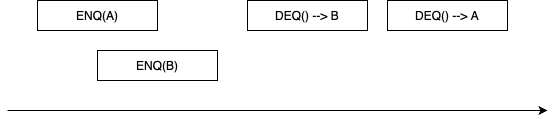
\includegraphics[width=4in]{good}
  \caption{An example of a linearizable execution. Both could take effect first since ENQ(A), and ENQ(B) are concurrent.}
\end{figure}

\begin{figure}[hbt]
  \center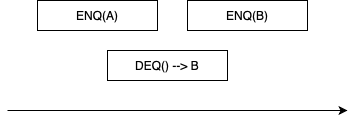
\includegraphics[width=3in]{bad}
  \caption{An example of an execution that is not linearizable. Since ENQ(A) has completed before ENQ(B) is invoked the DEQ() should return A.}
\end{figure}


An algorithm is \textit{wait-free} if each operation terminates after a finite number of steps. We call an algorithm \textit{lock-free} if, after a sufficient number of steps, one operation terminates. A wait-free algorithm is also lock-free. From now on, we are going to focus on wait freedom.

%Since executions on a shared data structure are different from sequential ones, the correctness condition also differs. The strongest correctness condition is linearizability, defined as "...". Lock-free is good, but a wait-free algorithm guarantees us every operation terminates after finite steps.

\paragraph{Previous Work}

In the following paragraphs, we look at previous work on distributed queues.
Michael \& Scott~\cite{DBLP:conf/podc/MichaelS96} introduced a lock-free queue which we refer to as the MS-queue. It is included in the standard Java Concurrency Package. Their idea is to store the queue in a singly~linked~list to compute the head and tail of the queue from the head and tail of the linked list. To insert a node to the linked list, they use compare and swap operations. If $p$ processes try to enqueue simultaneously, only one can succeed and the others have to retry. This makes the worst-case number of steps to be $\Omega(p)$ per enqueue. Similarly, dequeue can $\Omega(p)$ take steps.

Moir, Nussbaum, and Shalev~\cite{DBLP:conf/spaa/MoirNSS05} presented a more sophisticated queue by using the elimination idea. The elimination mechanism benefits the dual purpose of allowing operations to complete in parallel and reducing contention for the queue. An Elimination Queue consists of an MS-queue augmented with an elimination array. Elimination works by allowing opposing operations such as pushes and pops to exchange values. Their algorithm makes it possible for failed aged operations to complement. Empirical evaluation of their work is better than MS-queue, but the worst case is still the same, in case there are $p$ concurrent enqueus their algorithm is not better than MS-queue. 


Hoffman, Shalev, and Shavit~\cite{DBLP:conf/opodis/HoffmanSS07} tried to make the MS-queue more parallel by introducing the Baskets Queue. Their idea is to allow more parallelism by treating the simultaneous enqueue operations as a basket. Since the operations in a basket are concurrent, we can order them in any way. Operations in a basket try to find their position in queue one by one by using CAS operations. The operations in different baskets can be executed in parallel. However, like the previous algorithm, if still there are $p$ concurrent enqueue operations in a basket, the amortized complexity remains $\Omega(p)$.

Ladan-Mozes and Shavit~\cite{DBLP:journals/dc/Ladan-MozesS08} presented an Optimistic Approach to Lock-Free FIFO Queues. They use a doubly linked list and do fewer compare and swap operations than MS-queue. But as before, the worst case is when there are $p$ concurrent enqueues which have to be enqueued one by one. The amortized worst-case complexity is still $\Omega(p)$ CASes.

Hendler et al.~\cite{DBLP:conf/spaa/HendlerIST10} proposed a new paradigm called flat combining. Their queue is linearizable but not lock-free. After adding an operation acquiring the lock, they maintain history in publication records and compute all active operations responses. They believe their algorithm in real-world assumptions works well.

Gidenstam, Sundell and Tsigas~\cite{DBLP:conf/opodis/GidenstamST10} introduced a new algorithm using a linked list of arrays. Global head and tail point to arrays and content of arrays are marked if dequeued and written by CAS operations. Their data structure is lock-free but it updates lazily. Threads have a cache view on the queue and update it if it gets old.

Kogan and Perank~\cite{DBLP:conf/ppopp/KoganP11} introduced wait-free queues based on MS-queue and use Herlihy's helping technique to achieve wait-freeness. Their step complexity is $\Omega(p)$ because of the helping mechanism.

Milman et al.~\cite{DBLP:conf/spaa/MilmanKLLP18} designed BQ: A Lock-Free Queue with Batching. Their idea of batching allows a sequence of operations to be submitted as a batch for later execution. It supports a new notion introduced by the authors called Extended Medium Futures Linearizability.

Nikolaev and Ravindran~\cite{DBLP:journals/corr/abs-2201-02179} wCQ to be completed.



%FIFO queues have a wide range of use in OS and applications. The current state-of-the-art queues are implemented using linked lists; that's why they have factor p in their time complexity.

%\href{https://docs.google.com/spreadsheets/d/1cL1tgXXdljkh462sMwkTVMHH_k0MBTmslIVM3xA5VS4/edit#gid=0}{Table of previous works}

%There is a connection between queues and universal constructions. We can implement a universal construction using a queue. We can store operations in the shared queue and compute operations' responses using the queue's content. Some impractical universal constructions are using big words as "...".

\paragraph{Our contribution}
In this work, we are trying to design a queue with $\log p^2 +Q$ steps per operation, outperforming queues built by LinkedList. Our idea is similar to the Jayanti MESD queue.

\bibliography{main} 
\bibliographystyle{ieeetr}

\end{document}
